\documentclass[11pt]{article}
\usepackage[margin=0.95in]{geometry}
\usepackage{booktabs}
\usepackage{array}
\usepackage{longtable}
\usepackage{graphicx}
\usepackage{float}
\usepackage{amsmath,amssymb}
\usepackage{enumitem}
\usepackage{xcolor}
\usepackage{caption}
\usepackage{subcaption}
\usepackage{pdflscape}
\usepackage{hyperref}
\usepackage[numbers,sort&compress]{natbib}
\hypersetup{colorlinks=true,linkcolor=blue,citecolor=blue,urlcolor=blue}
\graphicspath{{../figures/}}

% Auto-generated from outputs/*.csv. Do not edit manually.
\newcommand{\CanonicalCells}{250}
\newcommand{\CanonicalModels}{41}
\newcommand{\CanonicalFamilies}{13}
\newcommand{\CanonicalBenchmarks}{12}
\newcommand{\CanonicalMAE}{9.28}
\newcommand{\CanonicalRMSE}{12.69}
\newcommand{\CanonicalBias}{-1.78}
\newcommand{\CanonicalRTwo}{0.64}
\newcommand{\CalibrationSlope}{0.89}
\newcommand{\TemporalMAE}{13.67}
\newcommand{\LOBOMAE}{12.76}
\newcommand{\CoveragePct}{50.8}
\newcommand{\StressMAELow}{8.87}
\newcommand{\StressMAEHigh}{9.87}
\newcommand{\BootstrapFullMAELow}{8.25}
\newcommand{\BootstrapFullMAEHigh}{10.37}
\newcommand{\BootstrapImprovementLow}{3.60}
\newcommand{\BootstrapImprovementHigh}{6.27}
\newcommand{\RecipeSensitivityLow}{9.20}
\newcommand{\RecipeSensitivityHigh}{12.30}
\newcommand{\AblationTable}{%
\begin{tabular}{lrrrrrl}\toprule
Specification & cells & families & scored & MAE & fold sd & status \\
\midrule
Scale & 250 & 13 & 250 & 14.14 & 3.55 & ok \\
Scale+Arch & 250 & 13 & 250 & 14.82 & 3.29 & ok \\
Scale+Recipe & 250 & 13 & 250 & 11.10 & 2.91 & ok \\
Full & 250 & 13 & 250 & 9.28 & 0.88 & ok \\
\bottomrule\end{tabular}}
\newcommand{\ResidualSummaryTable}{%
\begin{tabular}{lr}\toprule
Diagnostic & Value \\
\midrule
Cells & 250 \\
Weighted MAE & 9.28 pp \\
Weighted RMSE & 12.69 pp \\
Weighted bias & -1.78 pp \\
Weighted $R^2$ & 0.64 \\
Calibration slope & 0.89 \\
Calibration intercept & 5.64 \\
\bottomrule\end{tabular}}
\newcommand{\ValidationTable}{%
\begin{tabular}{lrrrrrrrr}\toprule
Validation & cells & models & families & benchmarks & MAE & RMSE & bias & $R^2$ \\
\midrule
family-grouped-CV & 250 & 41 & 13 & 12 & 9.28 & 12.69 & -1.78 & 0.64 \\
leave-one-family-out & 250 & 41 & 13 & 12 & 8.72 & 11.54 & -1.46 & 0.70 \\
leave-one-benchmark-out & 250 & 41 & 13 & 12 & 12.76 & 17.09 & 1.36 & 0.34 \\
temporal-holdout & 147 & 26 & 9 & 12 & 13.67 & 18.21 & -7.57 & -0.02 \\
\bottomrule\end{tabular}}
\newcommand{\BenchmarkResidualTable}{%
\begin{tabular}{lrrrrrr}\toprule
Benchmark & cells & models & MAE & RMSE & bias & p90 AE \\
\midrule
AIME\_2024 & 9 & 9 & 24.74 & 32.63 & -6.40 & 55.62 \\
GPQA\_Diamond & 25 & 25 & 12.53 & 14.78 & 2.03 & 20.90 \\
MATH & 33 & 33 & 12.10 & 14.02 & -4.40 & 19.79 \\
LiveCodeBench & 16 & 16 & 11.05 & 13.64 & 2.39 & 20.85 \\
ARC\_C & 18 & 18 & 10.49 & 13.22 & -4.54 & 21.62 \\
HumanEval & 28 & 28 & 8.81 & 11.34 & -2.98 & 19.74 \\
GSM8K & 23 & 23 & 7.98 & 12.32 & -4.81 & 22.68 \\
MMLU\_Pro & 22 & 22 & 7.46 & 9.35 & -0.80 & 15.15 \\
MBPP & 28 & 28 & 6.89 & 7.81 & -1.26 & 11.26 \\
IFEval & 9 & 9 & 6.68 & 8.63 & 2.06 & 11.73 \\
MMLU & 32 & 32 & 5.47 & 7.09 & -0.50 & 12.01 \\
BBH & 7 & 7 & 1.17 & 1.47 & -0.08 & 2.09 \\
\bottomrule\end{tabular}}
\newcommand{\FamilyResidualTable}{%
\begin{tabular}{lrrrrr}\toprule
Family & cells & models & MAE & bias & p90 AE \\
\midrule
GPT4 & 10 & 1 & 15.18 & -14.54 & 28.71 \\
Gemini & 6 & 4 & 15.17 & 11.51 & 19.73 \\
Llama3 & 24 & 4 & 12.21 & -11.63 & 26.29 \\
Gemma & 33 & 4 & 11.75 & -10.10 & 22.26 \\
Llama4 & 14 & 2 & 11.42 & 4.22 & 20.59 \\
Llama2 & 12 & 2 & 9.44 & 5.99 & 19.23 \\
Mistral & 20 & 3 & 8.98 & 2.71 & 17.89 \\
OpenAI\_o & 24 & 4 & 8.62 & 8.52 & 19.19 \\
Claude & 14 & 3 & 8.29 & -5.55 & 20.70 \\
Phi & 24 & 3 & 8.09 & 3.28 & 16.53 \\
\bottomrule\end{tabular}}
\newcommand{\SourceResidualTable}{%
\begin{tabular}{lrrrrr}\toprule
Source & cells & models & MAE & bias & p90 AE \\
\midrule
leaderboard & 6 & 1 & 9.66 & -4.27 & 18.48 \\
cross\_report & 38 & 8 & 9.50 & -3.27 & 18.99 \\
official & 202 & 33 & 9.33 & -1.54 & 20.33 \\
simple\_evals & 4 & 2 & 3.53 & 1.48 & 5.43 \\
\bottomrule\end{tabular}}
\newcommand{\OutlierTable}{%
\begin{tabular}{llrrrl}\toprule
Model & Benchmark & observed & predicted & residual & source \\
\midrule
GPT-4o & AIME\_2024 & 9.3 & 76.4 & -67.1 & cross\_report \\
Claude-3.5-Sonnet & AIME\_2024 & 16.0 & 68.8 & -52.8 & cross\_report \\
Gemma-3-4B-Base & GSM8K & 38.4 & 77.6 & -39.2 & official \\
o3-mini & AIME\_2024 & 87.3 & 48.3 & 39.0 & official \\
Llama-3.1-405B & MATH & 37.5 & 67.9 & -30.4 & official \\
DeepSeek-V3 & AIME\_2024 & 39.2 & 68.1 & -28.9 & official \\
Llama-3.1-8B & GSM8K & 50.0 & 76.6 & -26.6 & official \\
Llama-3.1-70B & MATH & 30.0 & 56.3 & -26.3 & official \\
Llama-3.1-8B & ARC\_C & 55.0 & 81.3 & -26.3 & official \\
Llama-3.1-8B & MATH & 15.8 & 41.3 & -25.5 & official \\
o3-mini & GPQA\_Diamond & 79.7 & 54.3 & 25.4 & official \\
Mistral-7B & GSM8K & 35.4 & 60.7 & -25.3 & leaderboard \\
GPT-4o & GPQA\_Diamond & 49.9 & 74.3 & -24.4 & cross\_report \\
Llama-2-7B & ARC\_C & 53.0 & 28.6 & 24.4 & official \\
Gemma-3-4B-Base & HumanEval & 36.0 & 60.2 & -24.2 & official \\
\bottomrule\end{tabular}}
\newcommand{\SensitivityTable}{%
\begin{tabular}{llllrrrl}\toprule
Source policy & scale & target & estimator & cells & families & MAE & status \\
\midrule
official\_only & continuous & logit & ridge & 202 & 11 & 8.35 & ok \\
official\_only & bucket & logit & ridge & 202 & 11 & 8.36 & ok \\
official\_like & bucket & logit & ridge & 250 & 13 & 8.58 & ok \\
full & bucket & logit & ridge & 308 & 14 & 8.82 & ok \\
full & continuous & logit & ridge & 308 & 14 & 9.16 & ok \\
official\_like & continuous & logit & ridge & 250 & 13 & 9.28 & ok \\
official\_like & continuous & raw & ridge & 250 & 13 & 10.14 & ok \\
\bottomrule\end{tabular}}
\newcommand{\CoefficientTable}{%
\begin{tabular}{llr}\toprule
Feature & group & standardized coefficient \\
\midrule
math\_intensity & training/recipe & 0.540 \\
bench\_LiveCodeBench & benchmark fixed effects & -0.397 \\
log\_active\_params & scale/capacity & 0.389 \\
release\_year\_norm & training/recipe & 0.321 \\
math\_intensity\_x\_outputspace & recipe x benchmark interactions & -0.309 \\
log\_context & architecture/context & -0.300 \\
contamination\_resistant & benchmark metadata & -0.297 \\
output\_space & benchmark metadata & 0.293 \\
is\_instruct & training/recipe & 0.258 \\
bench\_GSM8K & benchmark fixed effects & 0.246 \\
is\_reasoning\_model\_x\_outputspace & recipe x benchmark interactions & -0.242 \\
is\_reasoning\_model & training/recipe & 0.227 \\
thinking\_on\_cell & measurement/protocol & 0.227 \\
retained\_v22 & benchmark metadata & 0.203 \\
bench\_MMLU & benchmark fixed effects & 0.198 \\
synthetic\_quality\_x\_outputspace & recipe x benchmark interactions & -0.195 \\
bench\_MATH & benchmark fixed effects & -0.186 \\
bench\_BBH & benchmark fixed effects & 0.167 \\
n\_choices & benchmark metadata & 0.163 \\
bench\_ARC\_C & benchmark fixed effects & 0.160 \\
\bottomrule\end{tabular}}
\newcommand{\MissingSummaryTable}{%
\begin{tabular}{lr}\toprule
Diagnostic & Value \\
\midrule
Possible model-benchmark cells & 492 \\
Observed canonical cells & 250 \\
Coverage & 50.8\% \\
Descriptive missingness AUC & 0.76 \\
\bottomrule\end{tabular}}
\newcommand{\StressTable}{%
\begin{tabular}{lr}\toprule
Diagnostic & Value \\
\midrule
Iterations & 60 \\
Mean MAE & 9.36 pp \\
MAE standard deviation & 0.34 pp \\
5th--95th percentile MAE & 8.87--9.87 pp \\
\bottomrule\end{tabular}}
\newcommand{\BootstrapTable}{%
\begin{tabular}{lr}\toprule
Diagnostic & Value \\
\midrule
Bootstrap iterations & 1000 \\
Full-model MAE & 9.28 pp \\
Full-model 95\% CI & 8.25--10.37 pp \\
Scale-only MAE & 14.14 pp \\
Improvement over scale-only & 4.86 pp \\
Improvement 95\% CI & 3.60--6.27 pp \\
Bootstrap Pr(improvement $\leq$ 0) & 0.000 \\
\bottomrule\end{tabular}}
\newcommand{\RecipeSensitivityTable}{%
\begin{tabular}{lr}\toprule
Diagnostic & Value \\
\midrule
Perturbation iterations & 60 \\
Mean MAE & 10.66 pp \\
MAE standard deviation & 0.96 pp \\
5th--95th percentile MAE & 9.20--12.30 pp \\
Min--max MAE & 8.25--12.75 pp \\
\bottomrule\end{tabular}}
\newcommand{\TemporalTable}{%
\begin{tabular}{rrrrrrr}\toprule
Cutoff yr & train cells & test cells & test models & MAE & RMSE & bias \\
\midrule
2024.75 & 87 & 163 & 28 & 11.95 & 16.40 & 0.55 \\
2024.95 & 103 & 147 & 26 & 13.67 & 18.21 & -7.57 \\
2025.08 & 142 & 108 & 21 & 10.30 & 13.92 & -8.37 \\
2025.25 & 192 & 58 & 15 & 8.33 & 10.92 & -2.46 \\
\bottomrule\end{tabular}}


\title{Predictable Benchmarks?\\
An Evaluation-Protocol-Adjusted Residual Audit of Public LLM Benchmark Scores}
\author{Ed Herranz\\
\small Independent research draft}
\date{Data snapshot: May 2026}

\begin{document}
\maketitle

\begin{abstract}
Public large language model (LLM) leaderboards often present benchmark scores as directly comparable measurements of model capability. In practice, a reported benchmark score is also a measurement artifact: it depends on benchmark version, score scale, source type, prompt setting, reasoning or thinking mode, sampling policy, tool access, and publication conventions. This paper asks a limited but practically important question: how much of the variation in public LLM benchmark scores is predictable from public model metadata and observable evaluation-protocol covariates? We assemble a model-benchmark-source-protocol panel with \CanonicalCells{} primary percent-score cells, \CanonicalModels{} models, \CanonicalFamilies{} model families, and \CanonicalBenchmarks{} benchmark variants. The panel explicitly includes Gemini models and separates benchmark versions and score scales when they are not exchangeable, such as AIME 2024 versus AIME 2025 and LiveCodeBench percent scores versus LiveCodeBench Pro Elo.

The canonical evaluation-protocol-adjusted ridge model obtains a source-weighted family-grouped cross-validation mean absolute error (MAE) of \CanonicalMAE{} percentage points, compared with a scale-only MAE of approximately 14 percentage points. Stronger validation tests reveal the limits of the result: leave-one-benchmark-out and temporal holdout errors are materially larger, and only \CoveragePct{}\% of possible model-benchmark cells are observed. The main contribution is therefore not a new universal scaling law and not a claim about intelligence. The contribution is a reproducible residual-audit framework: public benchmark scores are substantially compressible using public metadata and measurement controls, while the residuals identify benchmark cells that deserve data, protocol, or model-specialization review.
\end{abstract}

\section{Introduction}
LLM evaluation has become a public ranking exercise. Model cards, technical reports, vendor blogs, and third-party leaderboards report scores on MMLU, GPQA, AIME, HumanEval, LiveCodeBench, and related tasks. These scores are often interpreted as direct evidence about model capability. That interpretation is useful only as a first approximation. A reported score is not generated by the model alone. It is produced by a model evaluated under a procedure: a benchmark version, a prompt or scaffold, an answer-extraction rule, a sampling policy, a tool policy, a reasoning-effort setting, and a reporting source.

This paper studies benchmark predictability as a measurement problem. If a public benchmark score can be predicted well from public model metadata, family lineage, training-recipe proxies, benchmark characteristics, and evaluation-protocol covariates, then the raw leaderboard entry may contain less independent evidence than it appears to contain. Conversely, residuals from such a model are useful. A large residual may indicate a genuinely distinctive capability, benchmark-specific tuning, evaluation-protocol mismatch, source inconsistency, stale data, or an error in model metadata. The residual is not automatically a discovery, but it is a practical review queue.

The paper is deliberately framed as a residual audit rather than a causal model. The analysis does not claim to estimate private training compute, prove data contamination, or measure general intelligence. It asks how much public leaderboard variation can be compressed using observable covariates, and which unexplained cells remain after that adjustment.

\paragraph{Contributions.} The paper makes four contributions. First, it defines an evaluation-protocol-adjusted observation unit for public benchmark scores. Second, it proposes a reproducible feature taxonomy covering model scale, architecture, training and post-training recipe proxies, source reliability, benchmark metadata, and protocol variables. Third, it evaluates the model under family-grouped, leave-one-family-out, leave-one-benchmark-out, temporal, and closed-source parameter-uncertainty stress tests. Fourth, it treats residual diagnostics as the main output, not as an afterthought.

\section{Related work and positioning}
The literature on neural scaling laws shows that language-model loss and downstream performance often vary smoothly with scale, data, and compute. Kaplan et al. fit empirical scaling laws for language modeling loss over many orders of magnitude in model size, data, and compute \citep{kaplan2020scaling}. Hoffmann et al. later showed that compute-optimal training requires scaling model size and training data together, implying that parameter count alone is not sufficient for interpreting performance \citep{hoffmann2022training}.

This paper is closest to work that predicts benchmark performance rather than loss. Epoch AI's benchmark-extrapolation work uses estimated loss from scaling laws and then maps loss into benchmark performance \citep{owen2023predictable}. Sloth, or Skills Scaling Laws, models multi-benchmark performance across model families using low-dimensional latent skills and public benchmark data \citep{polo2024sloth}. Those papers motivate the present study, but the contribution here is different. We do not introduce a new scaling law or latent-skill model. We instead ask whether reported public benchmark cells remain informative after conditioning on public metadata and evaluation-protocol variables.

The paper also relates to benchmark transparency and contamination research. HELM emphasizes transparent, multi-scenario evaluation rather than single-score ranking \citep{liang2022helm}. BIG-bench illustrates the value and difficulty of broad benchmark design \citep{srivastava2022bigbench}. LiveCodeBench was created partly to reduce contamination risk by continuously collecting new coding problems over time \citep{jain2024livecodebench}. Surveys of benchmark contamination emphasize that static public tests can overstate generalization when evaluation data appears in training data \citep{xu2024contamination}. The present paper does not test contamination directly. It treats contamination resistance and benchmark refresh properties as benchmark metadata and then asks whether residuals are larger or smaller after controlling for such metadata.

\section{Research questions}
The study is organized around four research questions:
\begin{enumerate}[leftmargin=*]
\item \textbf{Predictability:} How much of the variation in public percent-score benchmark cells can be predicted from public metadata and evaluation-protocol covariates?
\item \textbf{Incremental information:} Which benchmark families remain difficult to predict after conditioning on scale, family, recipe, and protocol variables?
\item \textbf{Robustness:} How sensitive is the result to source filters, score transformations, closed-source parameter uncertainty, and stronger validation splits?
\item \textbf{Governance use:} Can the largest residuals be used as a transparent review queue for data errors, protocol mismatch, or model specialization?
\end{enumerate}

\section{Data design}
\subsection{Observation unit}
The observation unit is a model-benchmark-source-protocol cell. The canonical dependent variable is a score on a 0--100 percent scale. Non-percent scores are retained in the provenance data but excluded from the canonical percent-score regression unless they can be put onto a comparable scale without changing the meaning of the measurement. For example, LiveCodeBench Pro Elo is not combined with LiveCodeBench percent accuracy.

Benchmark variants are separated when the task or reporting protocol differs materially. AIME 2024 and AIME 2025 are different benchmark variables. Likewise, score variants that differ by sampling policy, tool use, or thinking mode are not treated as interchangeable unless the source provides enough information to justify the comparison.

\subsection{Source policy}
The canonical sample uses an ``official-like'' source policy. It includes official model cards, first-party technical reports, recognized simple-evals style sources, and cross-reported benchmark tables when those cross-reports are traceable and protocol-compatible. Aggregator rows and weakly estimated rows are retained in the provenance file but excluded from the canonical analysis unless the source policy is relaxed.

Each row receives a source weight. Official rows receive the highest weight, cross-reports and recognized leaderboards receive intermediate weights, and weaker sources receive lower weights. These weights are pragmatic measurement weights, not truth labels. They prevent an informal aggregator row from having the same influence as a primary model-card result.

\subsection{Gemini inclusion and benchmark versioning}
Gemini is explicitly represented in the panel. Gemini 2.5 Pro and Gemini 2.5 Flash cells are sourced from the Gemini 2.5 technical report where comparable benchmark cells are available \citep{gemini25report}. Gemini 3 Pro and Gemini 3.1 Pro are included from Google DeepMind model-card reporting where benchmark version and score scale can be separated \citep{gemini31card}. The paper intentionally avoids mixing Gemini 3.1 Pro's LiveCodeBench Pro Elo score with percent-score LiveCodeBench rows. This is a concrete example of the evaluation-protocol-adjusted design: preserve the information, but do not force incompatible measurements into a single dependent variable. Gemini 3.5 was announced during the final packaging window, but it is not added to the canonical percent-score panel here because the available public announcement emphasizes newer agentic, coding, and multimodal benchmarks rather than a fully audited set of comparable canonical cells for this study \citep{gemini35blog}.

\subsection{Predictor taxonomy}
The predictors are divided into six classes.
\begin{enumerate}[leftmargin=*]
\item \textbf{Scale and capacity:} active parameter proxy, total parameter proxy, training-token proxy, scale bucket, mixture-of-experts flag, parameter-confidence score, and closed-source or imputation flags. Closed-source values are treated as noisy proxies.
\item \textbf{Architecture and context:} context length, dense versus mixture-of-experts structure, grouped-query attention flag, rotary-position-embedding flag, and other public architectural indicators.
\item \textbf{Training and post-training recipe proxies:} math intensity, code-pretraining intensity, synthetic-data quality, instruction tuning, reasoning-model flag, and release-era controls. These variables are ordinal codings from public documentation; they are not direct observations of private data mixtures.
\item \textbf{Evaluation-protocol variables:} source class, source weight, exact-protocol-match flag, thinking or reasoning mode, reasoning-effort indicator, tool-access flag, and score-scale compatibility.
\item \textbf{Benchmark metadata:} saturation proxy, output-space proxy, multiple-choice flag, contamination-resistance flag, and whether the benchmark is a legacy retained leaderboard task.
\item \textbf{Interactions:} selected recipe-by-benchmark-property interactions, allowing math, code, reasoning, and synthetic-data proxies to matter differently on open-form, refreshed, or contamination-resistant tasks.
\end{enumerate}

\section{Model formulation}
For percent-score benchmarks, the canonical target is a clipped logit transform:
\[
  z_{i b s p}=\log\left(\frac{\tilde y_{i b s p}}{1-\tilde y_{i b s p}}\right),
\]
where $y_{i b s p}$ is the reported percentage score for model $i$, benchmark $b$, source $s$, and protocol $p$, and $\tilde y$ is the score divided by 100 and clipped away from zero and one. Predictions are transformed back to percentage points before reporting MAE, RMSE, bias, and residuals.

The full pooled specification is
\[
 z_{i b s p}=\alpha_b + x_i'\beta + a_i'\eta + r_i'\rho + m_{s p}'\gamma + q_b'\delta
 + (r_i \otimes q_b)'\theta + \varepsilon_{i b s p},
\]
where $\alpha_b$ are benchmark fixed effects, $x_i$ contains scale predictors, $a_i$ architecture and context predictors, $r_i$ training and post-training recipe proxies, $m_{sp}$ source and evaluation-protocol variables, and $q_b$ benchmark metadata. The interaction term lets recipe variables differ by benchmark properties. The canonical estimator is ridge regression because the panel is sparse and the predictors are correlated. Coefficients should be interpreted as descriptive controls, not causal effects.

\section{Validation design}
The analysis uses five validation and stress-test regimes.
\begin{enumerate}[leftmargin=*]
\item \textbf{Family-grouped cross-validation:} model families are assigned to folds, so held-out predictions are not random cell splits from the same family. This is the canonical interpolation task.
\item \textbf{Leave-one-family-out:} each family is held out entirely. This tests whether the model generalizes to a family not observed during training.
\item \textbf{Leave-one-benchmark-out:} each benchmark is held out and benchmark fixed effects are disabled. This is a harder task that tests whether benchmark metadata generalizes to a benchmark not observed during training.
\item \textbf{Temporal holdout:} models after a release-date cutoff are predicted from earlier models. This approximates a forward-looking use case.
\item \textbf{Closed-source parameter uncertainty:} active-parameter, total-parameter, and training-token proxies are perturbed more heavily for closed-source or imputed rows. This tests fragility to uncertain scale inputs.
\end{enumerate}

\section{Results}
\subsection{Canonical accuracy and ablation}
\begin{table}[H]
\centering\small
\caption{Canonical family-grouped cross-validation accuracy by predictor set. MAE is source-weighted and reported in percentage points.}
\AblationTable
\label{tab:ablation}
\end{table}

\begin{figure}[H]
\centering
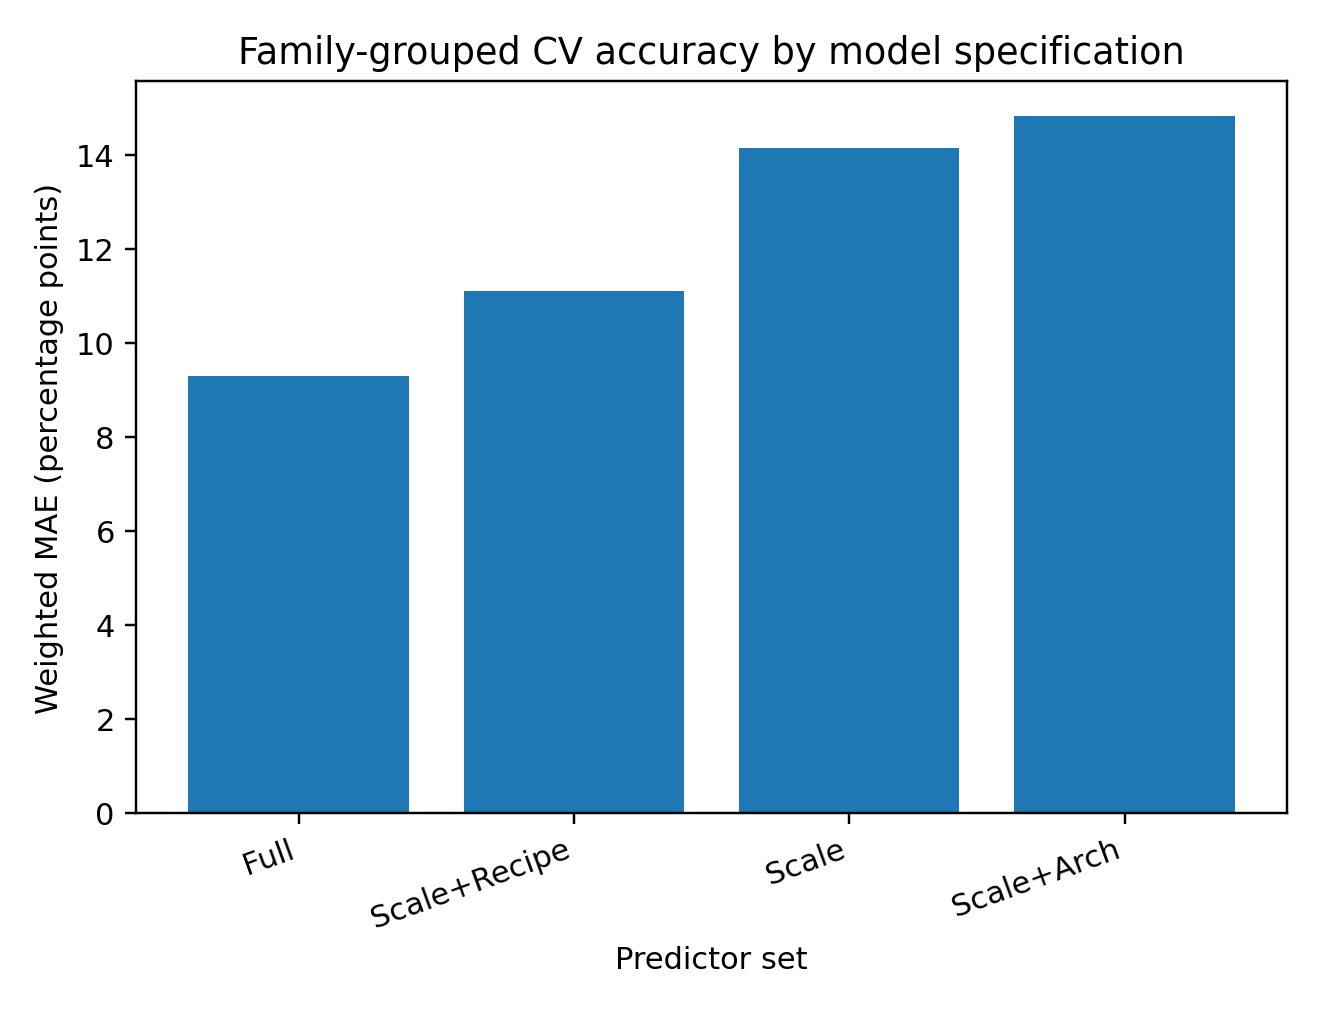
\includegraphics[width=0.72\textwidth]{accuracy_ablation.png}
\caption{Family-grouped cross-validation weighted MAE by predictor set. Lower is better.}
\label{fig:ablation}
\end{figure}

The full model obtains a source-weighted MAE of \CanonicalMAE{} percentage points, improving on the scale-only and scale-plus-recipe baselines. The result means that public benchmark scores are substantially compressible using public metadata and evaluation-protocol controls. It does not mean that the model has discovered a causal capability law.

\subsection{Calibration and prediction scatter}
\begin{figure}[H]
\centering
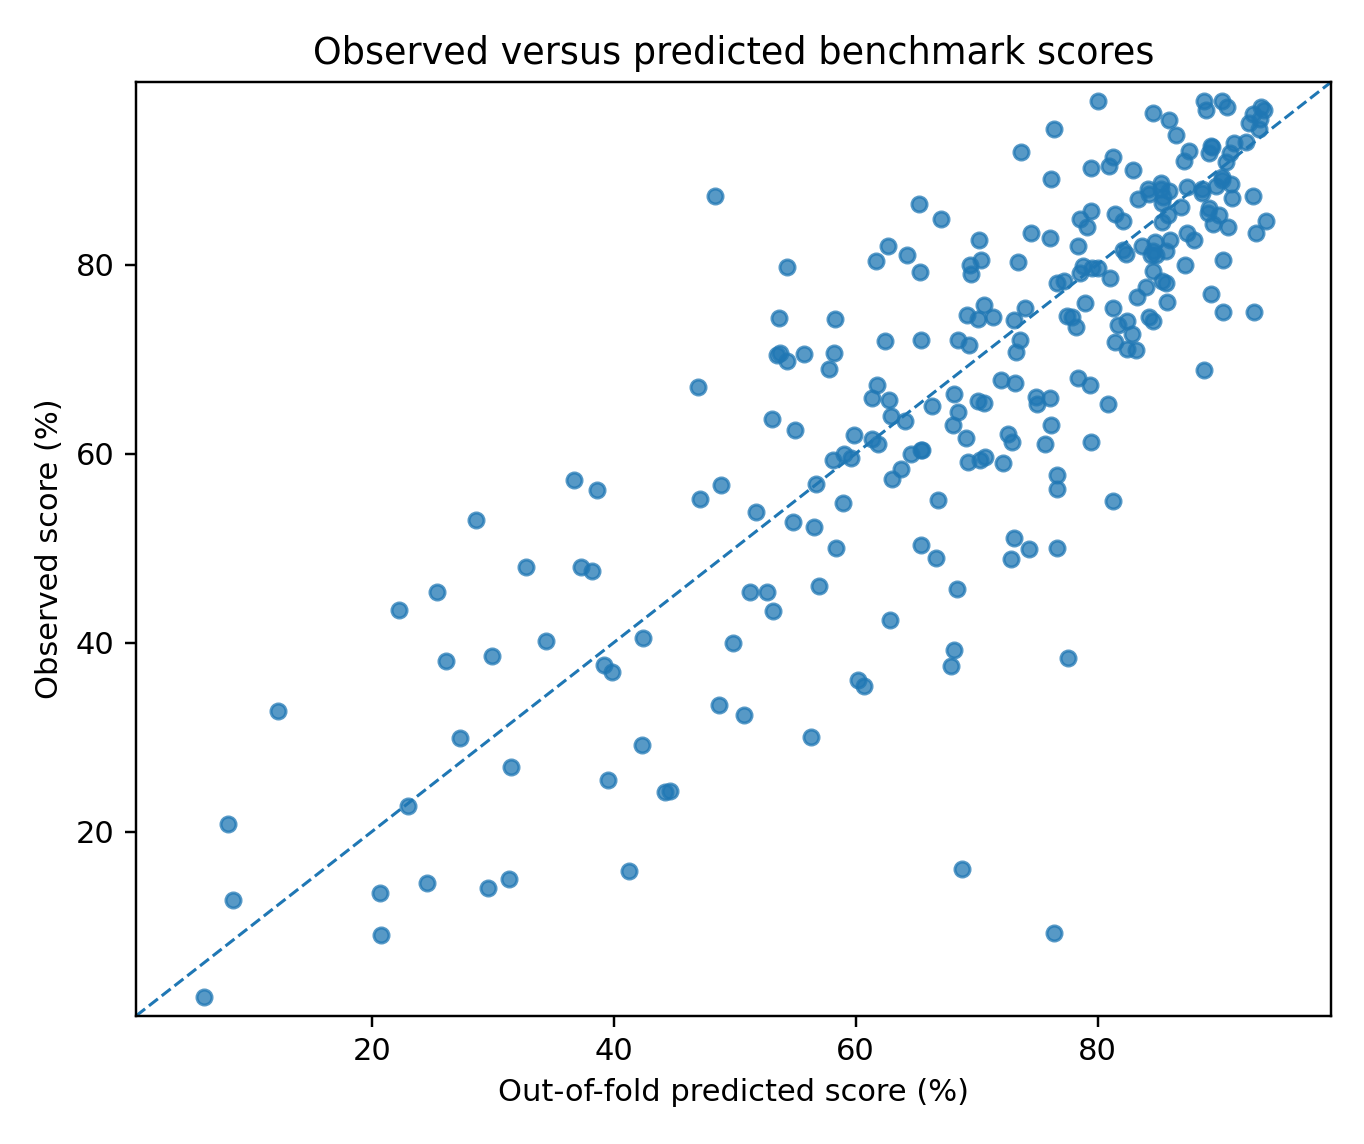
\includegraphics[width=0.72\textwidth]{observed_vs_predicted.png}
\caption{Observed versus out-of-fold predicted scores for the canonical full model. The purpose is residual audit, not certification of individual cells.}
\label{fig:obs_pred}
\end{figure}

\begin{table}[H]
\centering\small
\caption{Canonical residual diagnostics. Residual is observed minus predicted.}
\ResidualSummaryTable
\label{tab:res_summary}
\end{table}

The weighted bias is \CanonicalBias{} percentage points and the calibration slope is \CalibrationSlope{}. These diagnostics support use as a review tool, but the residual tails are too large for the model to validate individual leaderboard claims mechanically.

\section{Residual analysis}
Residuals are the central output of the study. A positive residual means the observed score is higher than predicted; a negative residual means the model overpredicted the reported score. Neither sign is automatically good or bad. Both can reflect genuine capability differences, protocol differences, source issues, or model-metadata errors.

\begin{figure}[H]
\centering
\begin{subfigure}{0.49\textwidth}
\centering
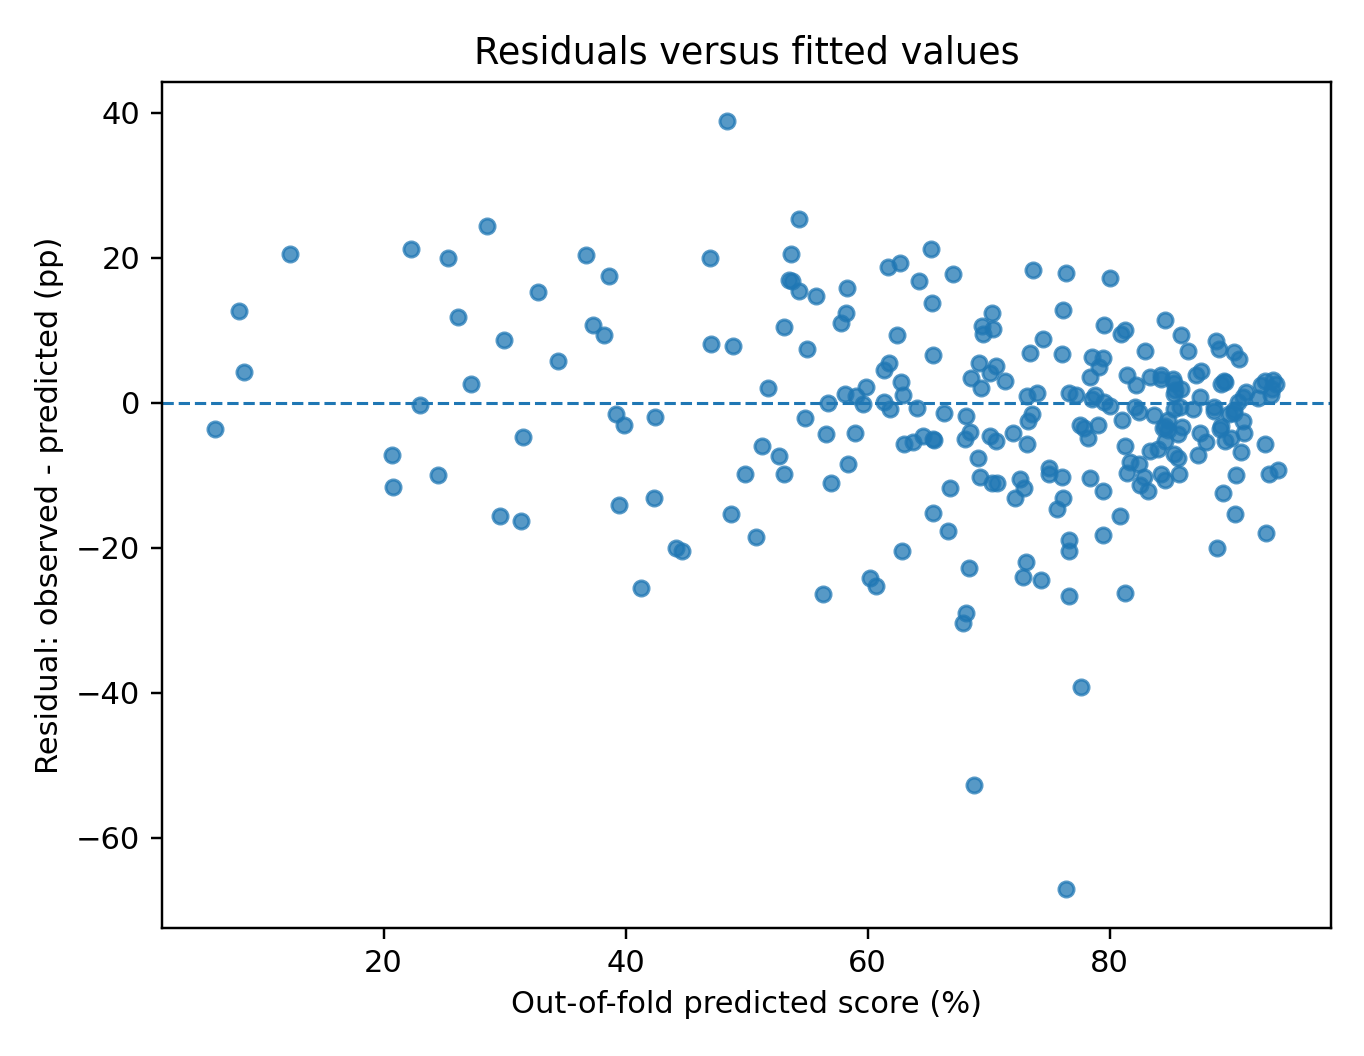
\includegraphics[width=\textwidth]{residuals_vs_fitted.png}
\caption{Residuals versus fitted values.}
\end{subfigure}
\begin{subfigure}{0.49\textwidth}
\centering
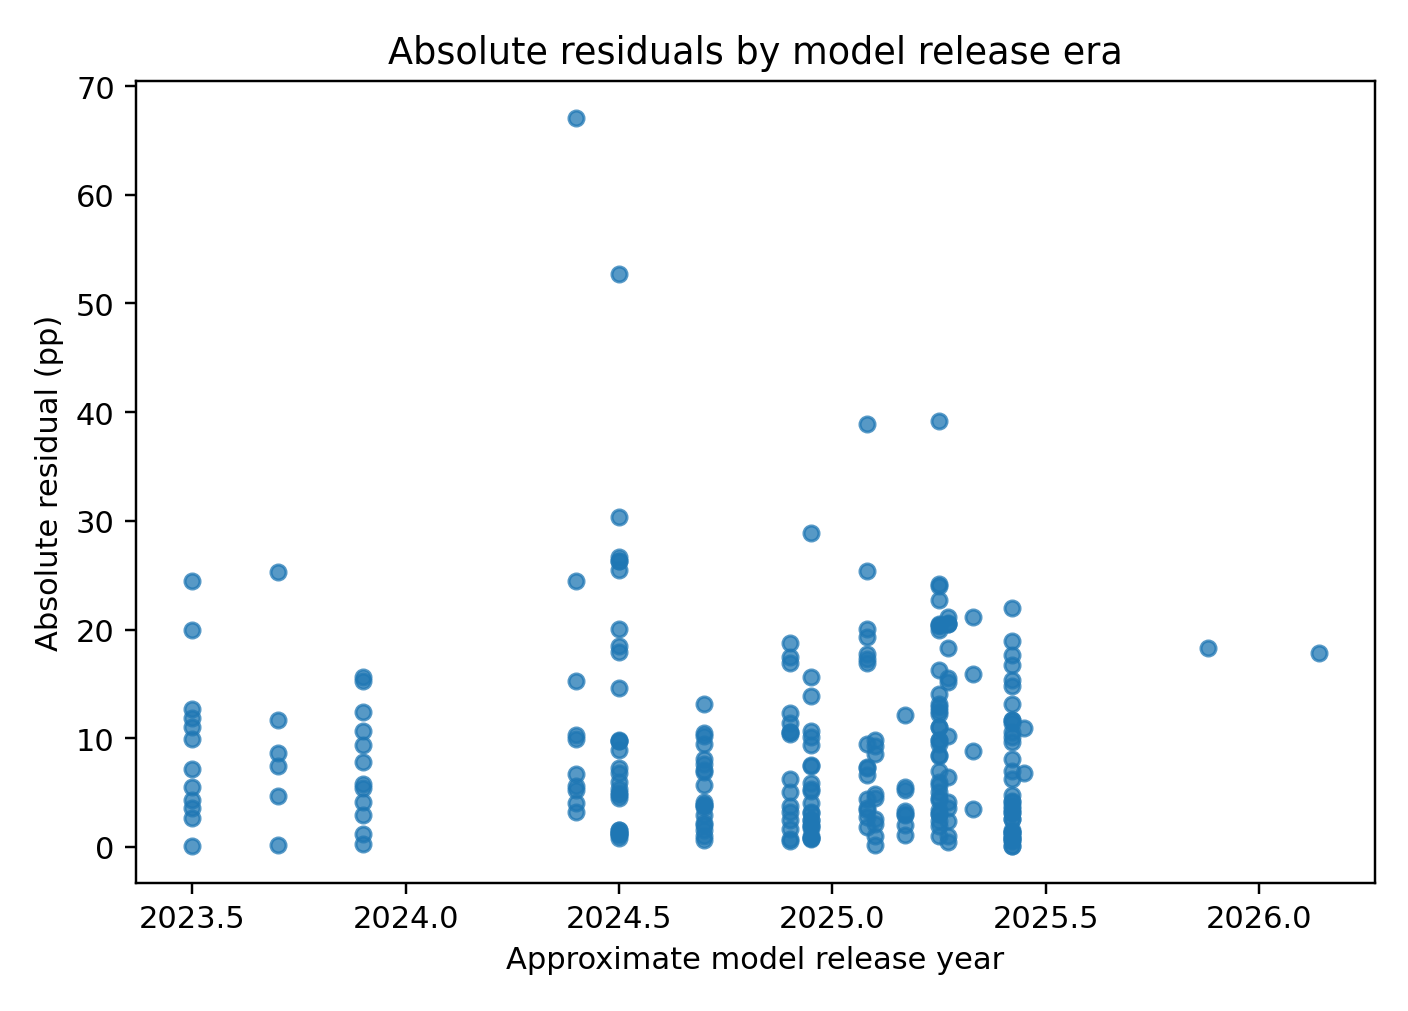
\includegraphics[width=\textwidth]{abs_residual_by_release.png}
\caption{Absolute residuals by release era.}
\end{subfigure}
\caption{Residual diagnostics by fitted score and release era.}
\label{fig:resids}
\end{figure}

\begin{figure}[H]
\centering
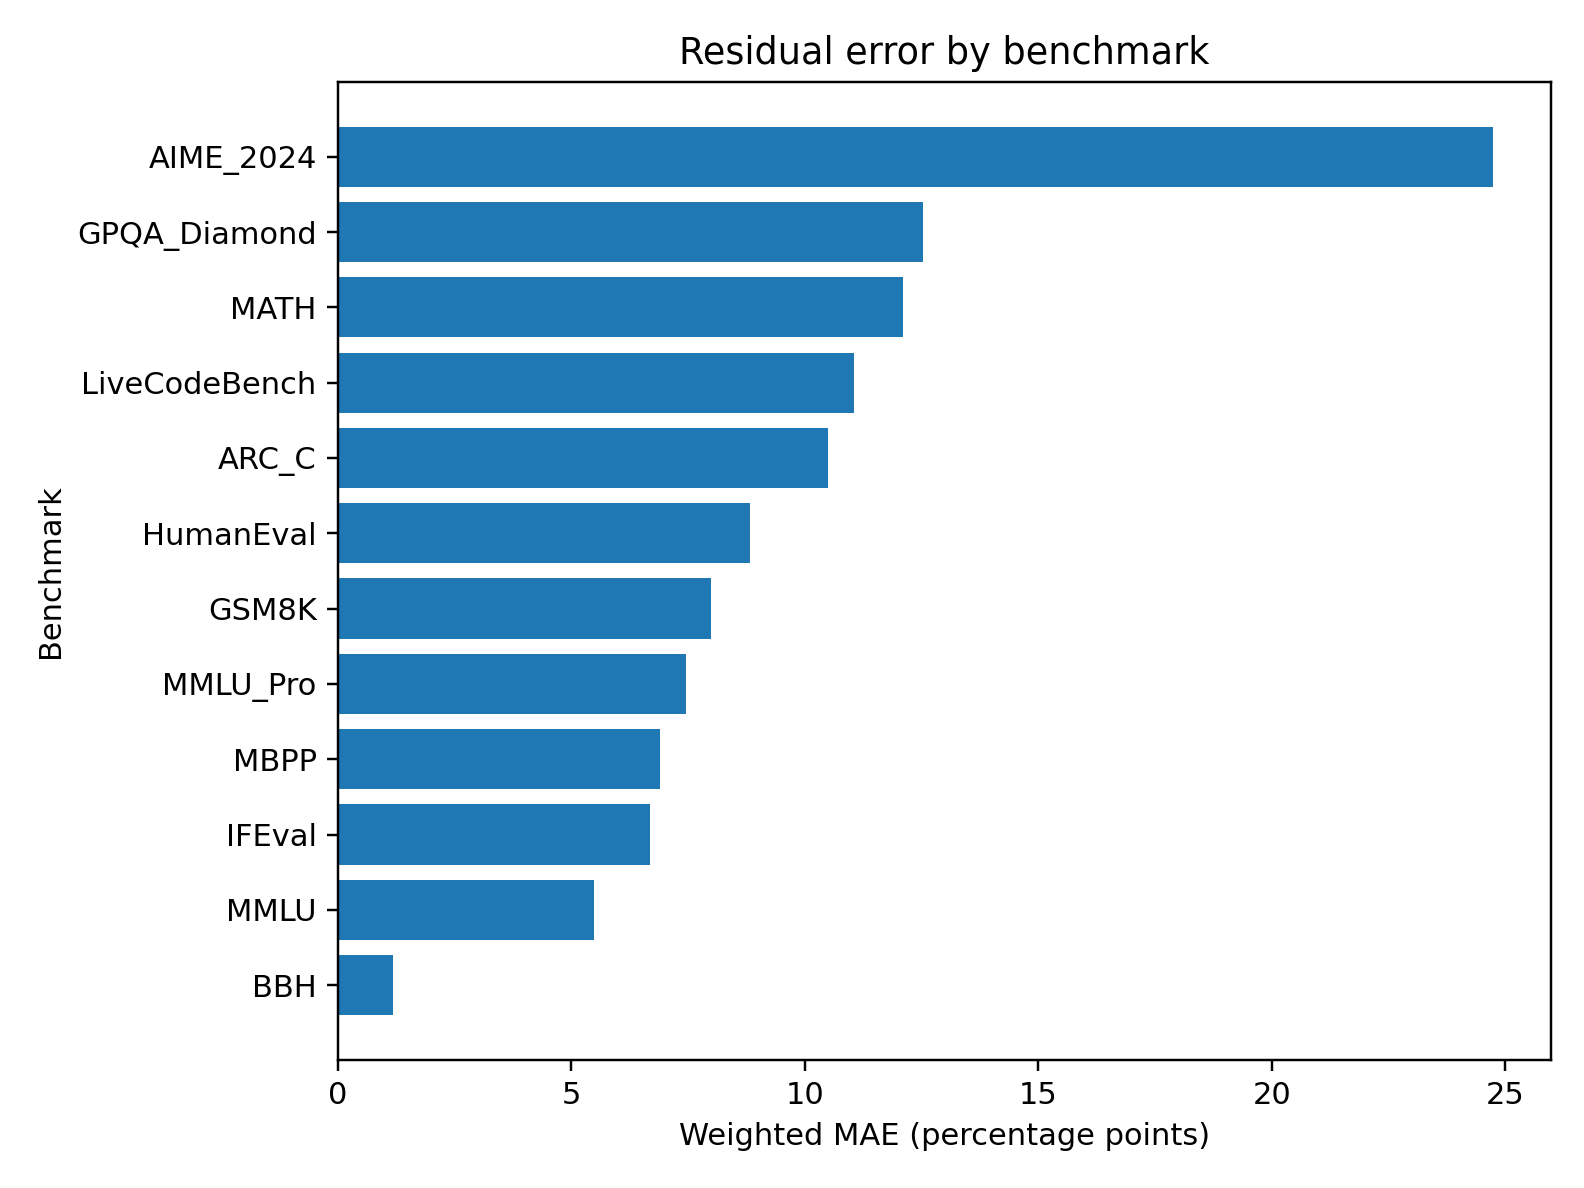
\includegraphics[width=0.82\textwidth]{mae_by_benchmark.png}
\caption{Weighted MAE by benchmark. Some benchmarks remain materially harder to predict after metadata and protocol adjustment.}
\label{fig:bench_mae}
\end{figure}

\begin{table}[H]
\centering\scriptsize
\caption{Residual diagnostics by benchmark. Positive bias means the model underpredicted the reported benchmark score.}
\resizebox{\textwidth}{!}{\BenchmarkResidualTable}
\label{tab:bench_residuals}
\end{table}

The benchmark residual table should be read together with sample size. BBH has only 7 cells and AIME\_2024 has only 9 cells in the canonical panel. These rows are useful as residual-review signals, but within-benchmark predictive claims for such rows are intentionally treated as sparse under the repository's minimum-model rule.

\begin{table}[H]
\centering\scriptsize
\caption{Largest family-level residual diagnostics.}
\resizebox{0.92\textwidth}{!}{\FamilyResidualTable}
\label{tab:family_residuals}
\end{table}

\begin{table}[H]
\centering\small
\caption{Residual diagnostics by source class.}
\SourceResidualTable
\label{tab:source_residuals}
\end{table}

\subsection{Outliers as a review queue}
\begin{table}[H]
\centering\scriptsize
\caption{Largest absolute out-of-fold residuals. These rows should be reviewed as data, protocol, or specialization cases before drawing substantive conclusions.}
\resizebox{\textwidth}{!}{\OutlierTable}
\label{tab:outliers}
\end{table}

The outlier table should not be read as an accusation list. It is a triage mechanism. For example, a large positive residual can indicate unusually strong model specialization, favorable test-time compute, or a missing covariate. A large negative residual can indicate a stale score, a stricter protocol, an overestimated scale proxy, or a benchmark-specific weakness.

\section{Robustness and limitations}
\subsection{Validation regimes}
\begin{figure}[H]
\centering
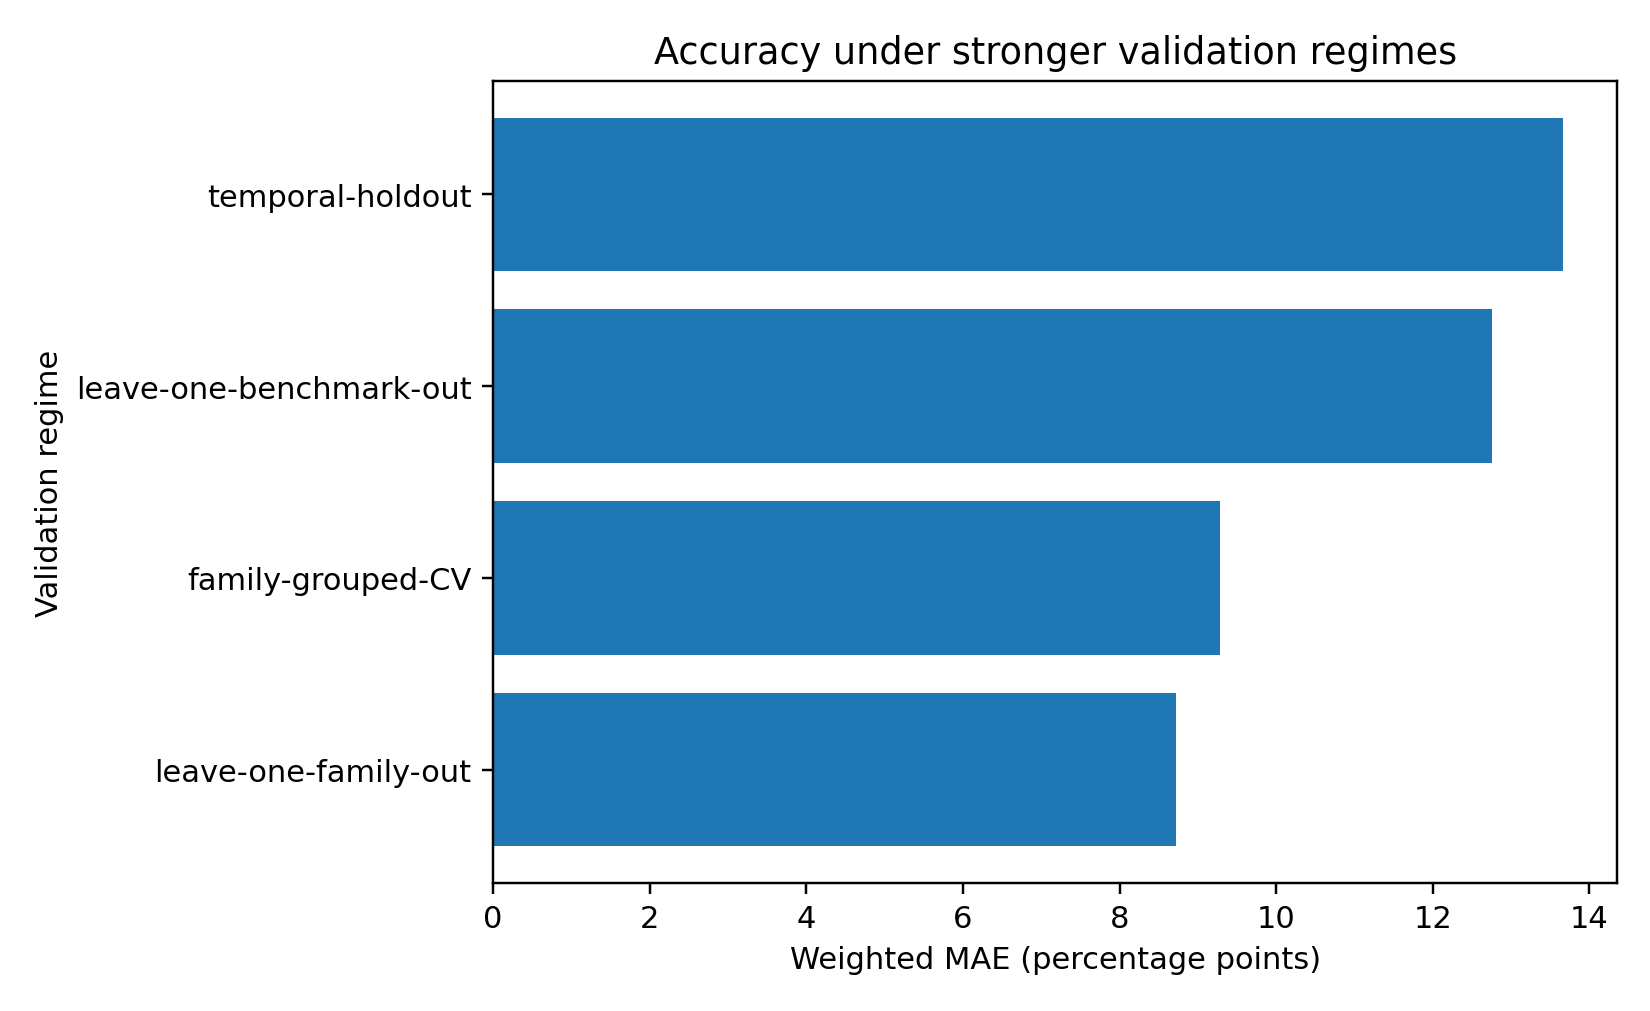
\includegraphics[width=0.82\textwidth]{validation_comparison.png}
\caption{Weighted MAE under stronger validation regimes. Leave-one-benchmark-out disables benchmark fixed effects, so it is not directly comparable to the canonical interpolation task.}
\label{fig:validation}
\end{figure}

\begin{table}[H]
\centering\scriptsize
\caption{Validation-regime comparison.}
\resizebox{\textwidth}{!}{\ValidationTable}
\label{tab:validation}
\end{table}

The temporal holdout MAE is \TemporalMAE{} percentage points and the leave-one-benchmark-out MAE is \LOBOMAE{} percentage points. The leave-one-benchmark-out value in Table~\ref{tab:validation} is the pooled weighted MAE across all held-out cells; the repository separately reports the unweighted mean of per-benchmark held-out fold MAEs. These larger errors are important. They show that the canonical result is strongest for interpolation among known benchmark families and known reporting conventions. Extrapolating to future models or unseen benchmarks remains substantially harder.

\begin{table}[H]
\centering\small
\caption{Paired bootstrap uncertainty for the canonical out-of-fold Full model and the Scale-only baseline. The bootstrap resamples prediction rows as intact pairs and recomputes source-weighted MAE.}
\BootstrapTable
\label{tab:bootstrap}
\end{table}

The paired bootstrap gives a 95\% interval of \BootstrapFullMAELow{}--\BootstrapFullMAEHigh{} percentage points for the full-model MAE and \BootstrapImprovementLow{}--\BootstrapImprovementHigh{} percentage points for the improvement over the scale-only baseline. This addresses sampling uncertainty in the observed cell panel, but it does not address unobserved benchmark cells or future protocol shifts.

\subsection{Missingness and closed-source parameter uncertainty}
\begin{figure}[H]
\centering
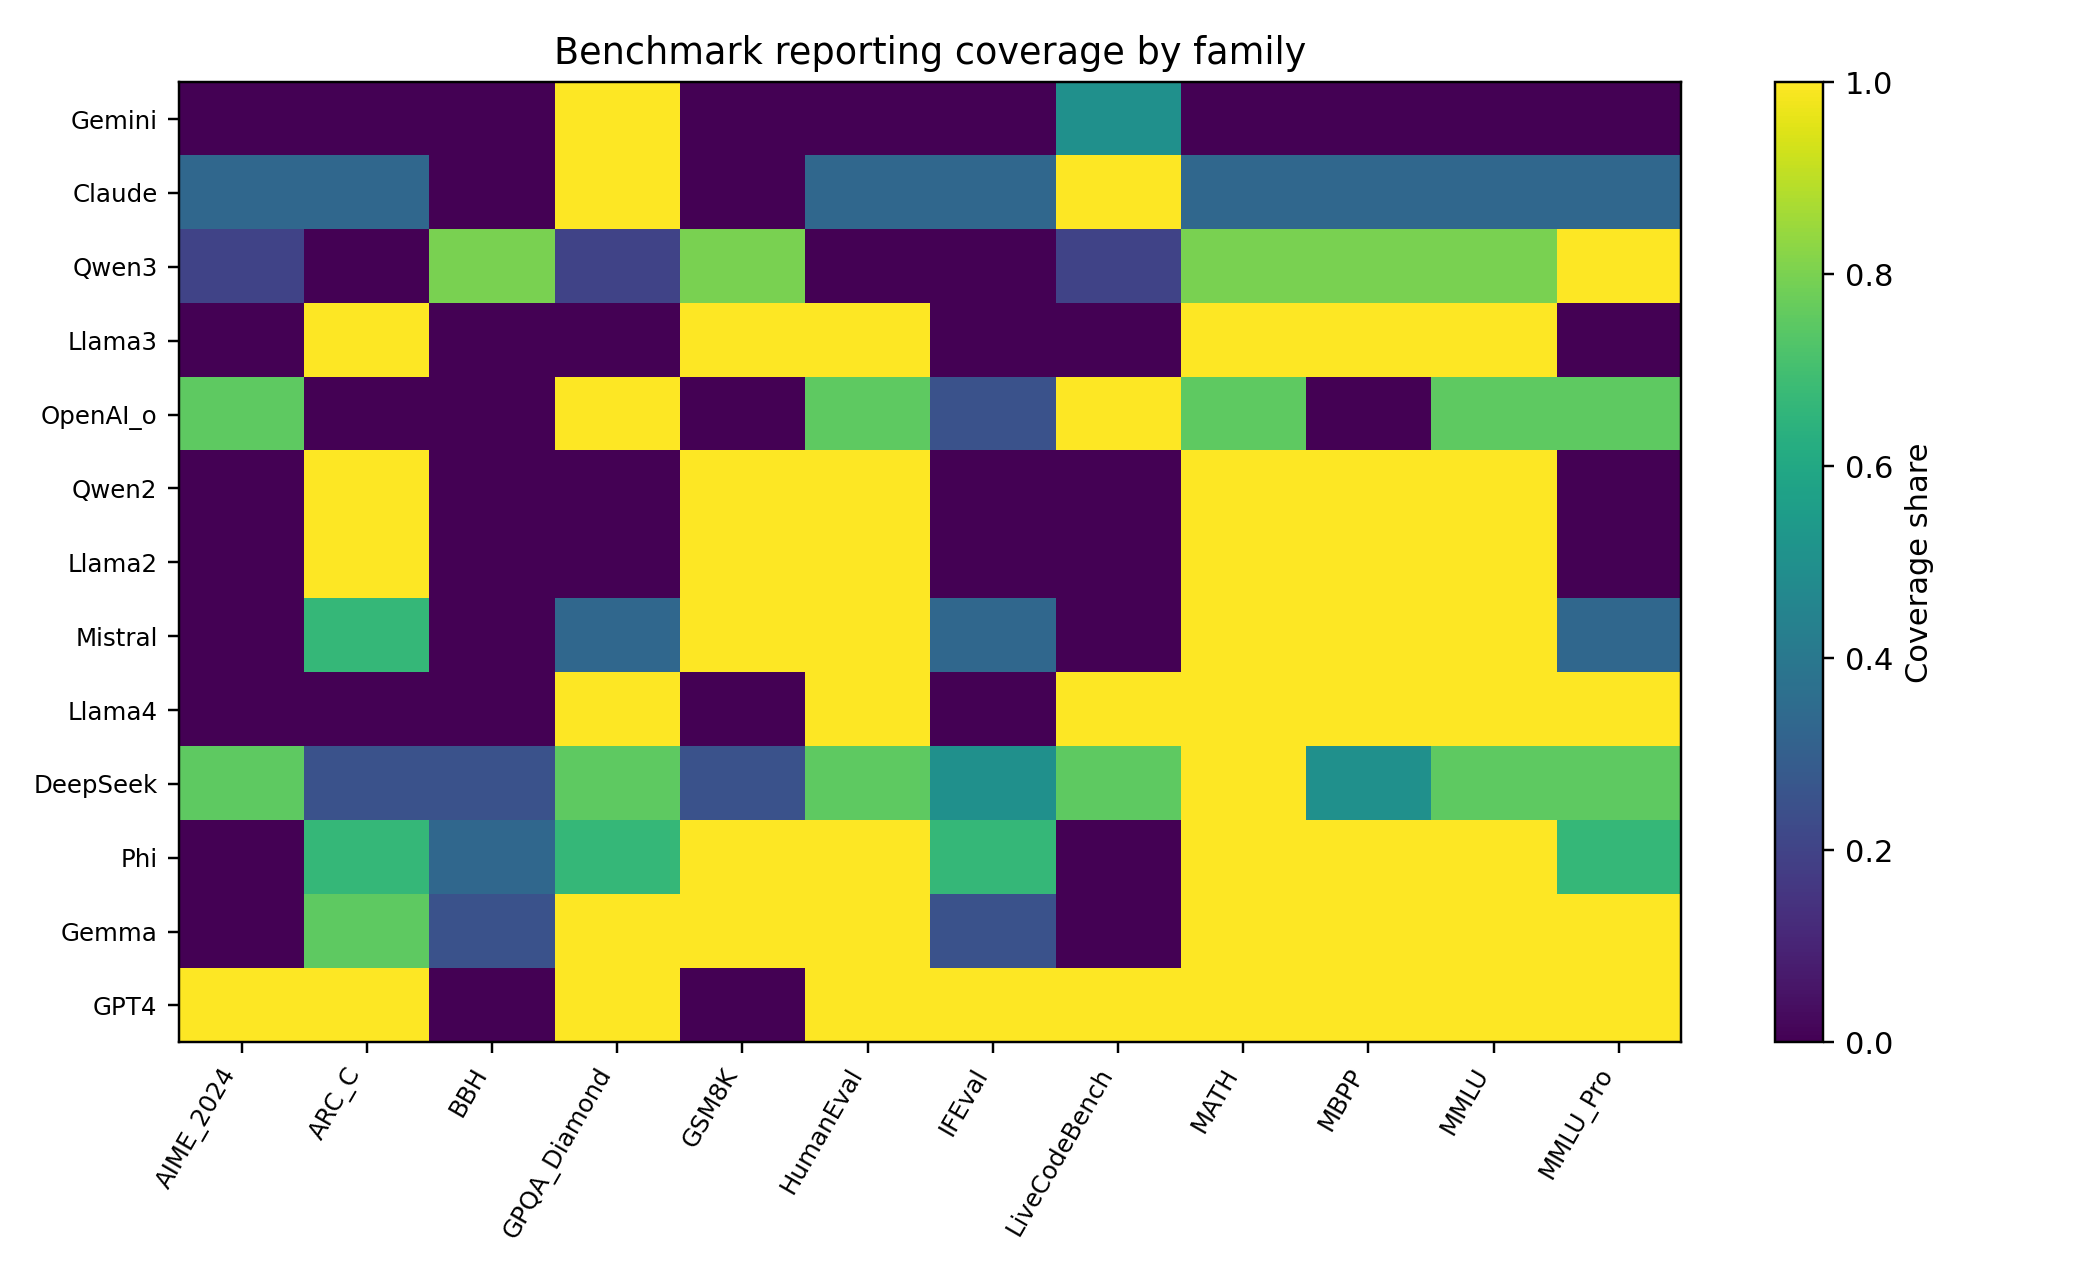
\includegraphics[width=0.82\textwidth]{missingness_heatmap.png}
\caption{Observed and missing model-benchmark cells in the canonical panel. Missingness is informative because vendors and evaluators do not report all benchmarks for all models.}
\label{fig:missingness}
\end{figure}

\begin{table}[H]
\centering\small
\caption{Missingness diagnostics.}
\MissingSummaryTable
\label{tab:missingness}
\end{table}

\begin{figure}[H]
\centering
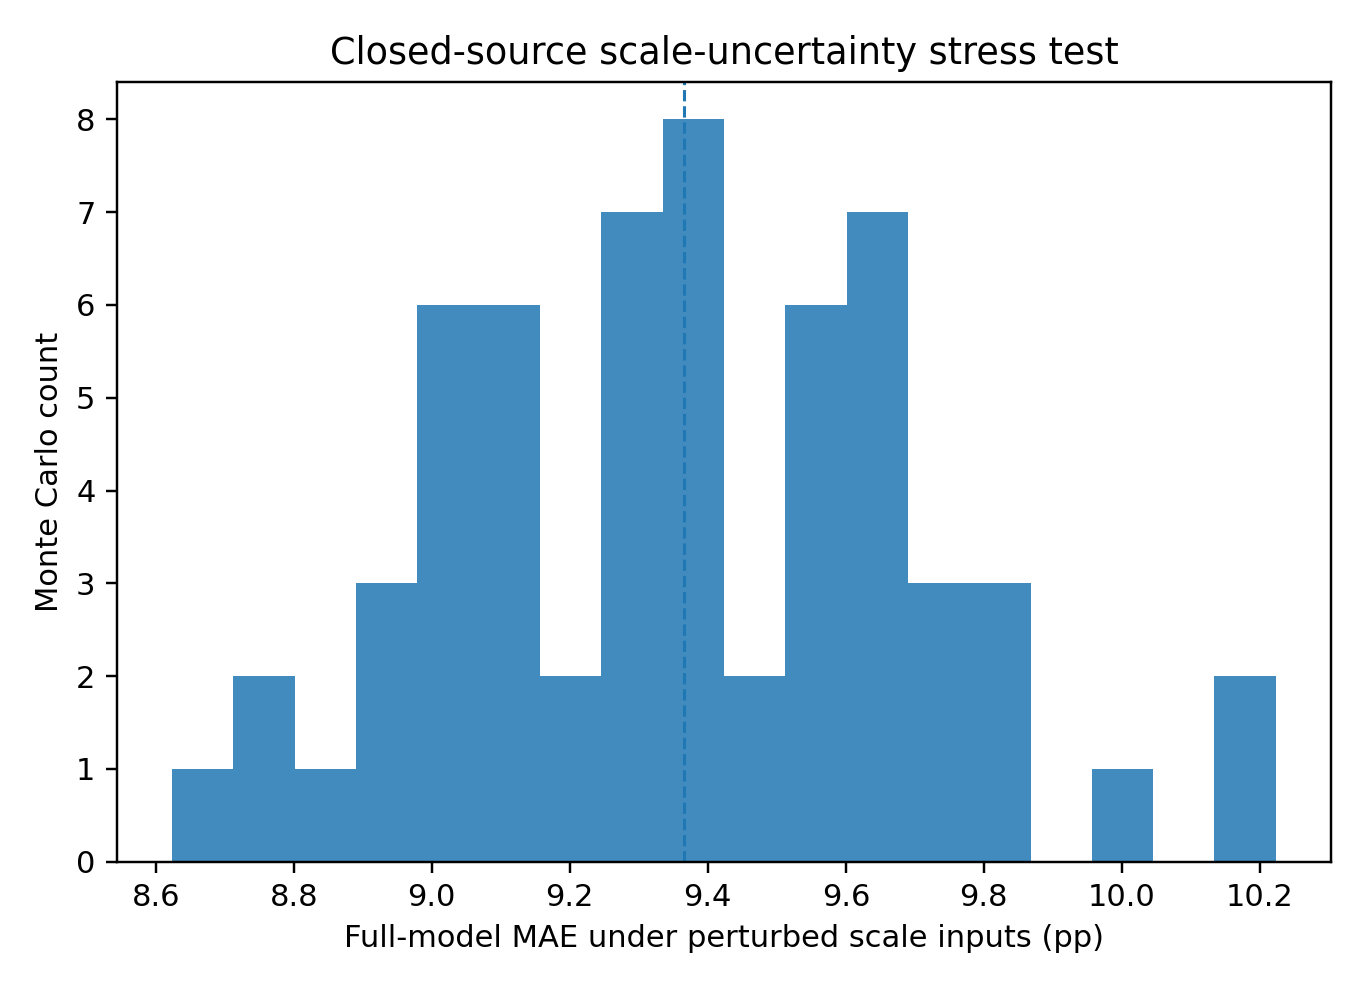
\includegraphics[width=0.72\textwidth]{param_uncertainty.png}
\caption{Closed-source parameter and token uncertainty stress test.}
\label{fig:param_uncertainty}
\end{figure}

\begin{table}[H]
\centering\small
\caption{Closed-source parameter and training-token perturbation stress test.}
\StressTable
\label{tab:stress}
\end{table}

The stress-test MAE range of \StressMAELow{}--\StressMAEHigh{} percentage points suggests that the headline fit is not dominated by one exact closed-source parameter assumption. However, the exercise is only a perturbation analysis; it does not recover true private training compute.

\subsection{Sensitivity grid}
\begin{table}[H]
\centering\scriptsize
\caption{Best full-model sensitivity settings among the grid runs.}
\resizebox{\textwidth}{!}{\SensitivityTable}
\label{tab:sensitivity}
\end{table}

The sensitivity grid supports the direction of the main result, but it also confirms that source policy, target transformation, and scale handling change the magnitude of the error. This is one reason the paper emphasizes residual review instead of a single universal accuracy number.

\begin{table}[H]
\centering\small
\caption{Sensitivity to one-step perturbations of the hand-coded ordinal recipe variables. Each iteration perturbs model-level math-intensity, code-pretraining, and synthetic-quality codes by -1, 0, or +1, clipped to the 0--2 coding range.}
\RecipeSensitivityTable
\label{tab:recipe_sensitivity}
\end{table}

The perturbation range of \RecipeSensitivityLow{}--\RecipeSensitivityHigh{} percentage points is a useful guardrail because the largest standardized recipe coefficient is not a directly observed quantity. The sensitivity does not remove the judgmental nature of the coding, but it makes the dependence on exact ordinal labels auditable.

\section{Threats to validity}
This study has several limitations that should be explicit in any publication.
\begin{enumerate}[leftmargin=*]
\item \textbf{Public metadata is incomplete.} Closed-source parameter counts, token counts, data composition, synthetic-data use, and post-training recipes are often approximate or inferred.
\item \textbf{Recipe variables are hand-coded.} Math intensity, code-pretraining intensity, and synthetic-data quality are ordinal 0--2 review variables, not measurements of private mixtures. The repository publishes the per-model coding table and a one-step perturbation sensitivity to make this limitation auditable.
\item \textbf{Protocol variables are coarse.} The model includes thinking mode, tool use, reasoning effort, and source class, but it does not observe exact prompts, hidden system instructions, routing behavior, verifier use, or answer-extraction details.
\item \textbf{Missingness is non-random.} The panel observes only about \CoveragePct{}\% of possible model-benchmark cells. Vendors and evaluators selectively report benchmarks.
\item \textbf{Benchmark fixed effects aid interpolation.} The canonical model uses benchmark fixed effects. Leave-one-benchmark-out results show that generalizing to unseen benchmarks is harder.
\item \textbf{Residuals are ambiguous.} A large residual is not automatically evidence of contamination, benchmark-specific training, or a data error. It is a prompt for review.
\item \textbf{The dataset is a snapshot.} LLM benchmark reporting changes quickly. New models and revised protocols should be added as new versioned rows rather than overwriting historical cells.
\end{enumerate}

\section{Reproducibility and code availability}
The accompanying repository contains the provenance data, feature definitions, analysis code, generated outputs, figures, and this paper. The intended public structure is:
\begin{verbatim}
data/      benchmark provenance and data dictionary
src/       analysis code and feature definitions
outputs/   generated CSV diagnostics and model outputs
figures/   generated figures used in the paper
paper/     LaTeX source and bibliography
scripts/   one-command reproduction helper
tests/     data-integrity checks
\end{verbatim}
The canonical command is \texttt{python src/run\_analysis.py}. The code is designed for reproducibility and auditability rather than for maximum predictive performance. Generated outputs and figures are committed as the release snapshot, while LaTeX build intermediates are ignored.

\paragraph{Public release.} The code, data, generated outputs, figures, and this manuscript are publicly available at \url{https://github.com/edherranz/llm-benchmark-residual-audit} and permanently archived at \url{https://doi.org/10.5281/zenodo.XXXXXXX}. The Zenodo concept DOI always resolves to the latest released version; per-release versioned DOIs are listed on the Zenodo record.

\paragraph{AI-use disclosure.} Generative AI tools were used to assist with drafting, code refactoring, diagnostic suggestions, LaTeX editing, and review of wording. The author reviewed, edited, and takes responsibility for the paper, data choices, code, and conclusions. AI assistance was not treated as an external source of factual benchmark data; benchmark values and citations are recorded in the provenance files and bibliography.

\paragraph{Affiliation and responsibility.} This is an independent research draft. Any institutional affiliation should be added only after confirming the applicable employer or institutional publication policy. The analysis and conclusions should not be attributed to any employer unless expressly approved.

\section{Conclusion: empirical surprises and implications}
Public benchmark scores are not independent, protocol-free measurements of model capability. In this dataset, a substantial portion of benchmark variation is predictable from public model metadata and observable evaluation-protocol variables. That does not make the benchmarks useless. It changes how they should be read. Raw leaderboard scores should be supplemented by residual analysis, source and protocol metadata, missingness diagnostics, and versioned benchmark definitions. The most informative benchmark entries may be the ones that remain surprising after the obvious metadata and measurement controls have been accounted for.

For this model and benchmark panel, the five most important empirical surprises are the following.
\begin{enumerate}[leftmargin=*]
\item \textbf{Leaderboard scores are more compressible than expected.} The full evaluation-protocol-adjusted model reduces weighted MAE from 14.14 percentage points for the scale-only baseline to \CanonicalMAE{} percentage points. Public metadata, benchmark identity, training-recipe proxies, and reporting-protocol covariates therefore explain a large share of apparent leaderboard variation.
\item \textbf{Residual difficulty is concentrated rather than diffuse.} AIME\_2024 has the largest benchmark-level MAE, \mbox{24.74} percentage points, while several older or more saturated benchmarks are much easier to predict. The largest AIME residuals separate pre-reasoning-era general models from explicitly reasoning-oriented models, suggesting that benchmark version, reasoning protocol, and release era cannot be treated as secondary details.
\item \textbf{Gemini is a real stress test for the framework, not merely an added row.} In the current snapshot, Gemini is among the most informative family-level residual cases. The Gemini cells show relatively large positive residuals, but the sample is small. The appropriate conclusion is therefore not that Gemini is categorically under- or over-valued; it is that official Gemini cells should remain versioned and protocol-separated, especially when LiveCodeBench Pro Elo and percent-score benchmarks coexist.
\item \textbf{The model is much stronger as an audit tool than as a forecasting engine.} The headline family-grouped result is materially weaker under leave-one-benchmark-out and temporal holdout validation. The model is useful for auditing known benchmark regimes, but it should not be sold as a reliable predictor for unseen benchmarks or future evaluation conventions.
\item \textbf{Selective reporting and protocol heterogeneity appear more important than modest closed-source scale uncertainty.} Only \CoveragePct{}\% of possible model-benchmark cells are observed, and missingness is predictable. By contrast, the closed-source parameter stress test moves MAE only within a narrow range of \StressMAELow{}--\StressMAEHigh{} percentage points. In this panel, the structure of what is reported, how it is reported, and under what protocol is a central part of the empirical object.
\end{enumerate}

The publication value of the study is therefore not the claim that architecture or parameter count mechanically determines capability. The stronger claim is methodological: once scale, family lineage, training-recipe proxies, benchmark metadata, source class, and evaluation protocol are accounted for, the residuals become the scientifically interesting object. They identify the benchmarks that still contain incremental information, the model families that do not fit the usual metadata pattern, and the cells where benchmark versioning, reporting protocol, or specialization should be reviewed before leaderboard differences are interpreted as capability differences.
\appendix
\section{Feature-coding rubric and model-level coding table}
The repository includes \texttt{docs/FEATURE\_CODING\_RUBRIC.md} and \texttt{data/model\_feature\_coding.csv}. The latter records the model-level family, scale proxies, confidence flags, MoE flag, reasoning-model flag, instruction flag, ordinal recipe codes, release year, and scale bucket used by the analysis. Closed-source scale entries should be read as low-confidence anchors, not parameter-count claims.

\section{Standardized coefficient summary}
\begin{table}[H]
\centering\scriptsize
\caption{Largest standardized coefficients in the canonical full model. Coefficients are descriptive because predictors are correlated and regularized.}
\resizebox{0.95\textwidth}{!}{\CoefficientTable}
\label{tab:coefficients}
\end{table}

\section{Temporal holdout details}
\begin{table}[H]
\centering\small
\caption{Temporal holdout splits.}
\TemporalTable
\label{tab:temporal}
\end{table}


\begin{thebibliography}{99}

\bibitem[Kaplan et~al.(2020)]{kaplan2020scaling}
Kaplan, J., McCandlish, S., Henighan, T., Brown, T. B., Chess, B., Child, R., Gray, S., Radford, A., Wu, J., and Amodei, D. (2020).
\newblock Scaling laws for neural language models.
\newblock \emph{arXiv:2001.08361}.

\bibitem[Hoffmann et~al.(2022)]{hoffmann2022training}
Hoffmann, J., Borgeaud, S., Mensch, A., Buchatskaya, E., Cai, T., Rutherford, E., de Las Casas, D., et~al. (2022).
\newblock Training compute-optimal large language models.
\newblock \emph{Advances in Neural Information Processing Systems}.

\bibitem[Polo et~al.(2024)]{polo2024sloth}
Polo, F. M., Somerstep, S., Choshen, L., Sun, Y., and Yurochkin, M. (2024).
\newblock Sloth: Scaling laws for LLM skills to predict multi-benchmark performance across families.
\newblock \emph{arXiv:2412.06540}.

\bibitem[Owen(2023)]{owen2023predictable}
Owen, D. (2023).
\newblock How predictable is language model benchmark performance?
\newblock Epoch AI blog and working paper.

\bibitem[Liang et~al.(2022)]{liang2022helm}
Liang, P., Bommasani, R., Lee, T., Tsipras, D., Soylu, D., Yasunaga, M., Zhang, Y., Narayanan, D., Wu, Y., Kumar, A., et~al. (2022).
\newblock Holistic evaluation of language models.
\newblock \emph{arXiv:2211.09110}.

\bibitem[Srivastava et~al.(2022)]{srivastava2022bigbench}
Srivastava, A., Rastogi, A., Rao, A., Shoeb, A. A. M., Abid, A., Fisch, A., Brown, A. R., Santoro, A., Gupta, A., Garriga-Alonso, A., et~al. (2022).
\newblock Beyond the imitation game: Quantifying and extrapolating the capabilities of language models.
\newblock \emph{arXiv:2206.04615}.

\bibitem[Jain et~al.(2024)]{jain2024livecodebench}
Jain, N., Han, K., Gu, A., Li, W.-D., Yan, F., Zhang, T., et~al. (2024).
\newblock LiveCodeBench: Holistic and contamination-free evaluation of large language models for code.
\newblock \emph{arXiv:2403.07974}.

\bibitem[Xu et~al.(2024)]{xu2024contamination}
Xu, C., Guan, S., Greene, D., and Kechadi, M.-T. (2024).
\newblock Benchmark data contamination of large language models: A survey.
\newblock \emph{arXiv:2406.04244}.

\bibitem[Google DeepMind(2025)]{gemini25report}
Google DeepMind. (2025).
\newblock Gemini 2.5 technical report.
\newblock Technical report.

\bibitem[Google DeepMind(2026)]{gemini31card}
Google DeepMind. (2026).
\newblock Gemini 3.1 Pro model card.
\newblock Model card.

\bibitem[Google DeepMind(2026b)]{gemini35blog}
Google DeepMind. (2026b).
\newblock Gemini 3.5: Frontier intelligence with action.
\newblock Google Keyword blog announcement.

\bibitem[OpenAI(2025)]{openai2025gpt5}
OpenAI. (2025).
\newblock Introducing GPT-5.
\newblock Product and technical announcement.

\bibitem[Anthropic(2026)]{anthropic2026sonnet46}
Anthropic. (2026).
\newblock Claude Sonnet 4.6 system card.
\newblock System card.

\end{thebibliography}

\end{document}
